\begin{block}{Results}
\begin{columns}
\begin{column}{.5\textwidth}
    These results show the expected/Standard Model values.
    The method works equally well for non-SM data.
    \begin{figure}
    \begin{minipage}{0.94\textwidth}
        \centering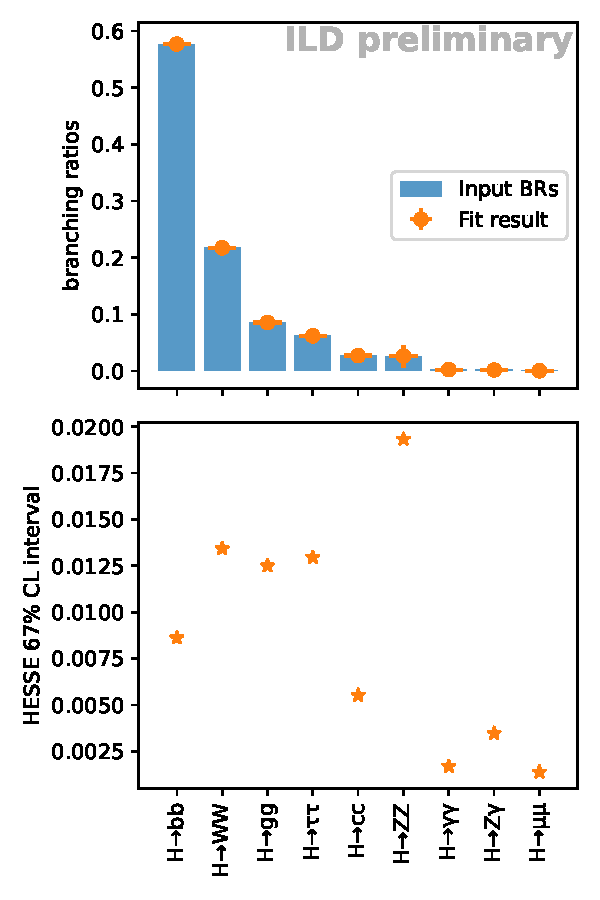
\includegraphics[width=0.9\textwidth]{br_estimates}
        \caption{Higgs branching ratios and their uncertainty.}
    \end{minipage}
    \end{figure}
\end{column}
\begin{column}{.3\textwidth}
    \begin{figure}
    \begin{minipage}{0.94\textwidth}
        \centering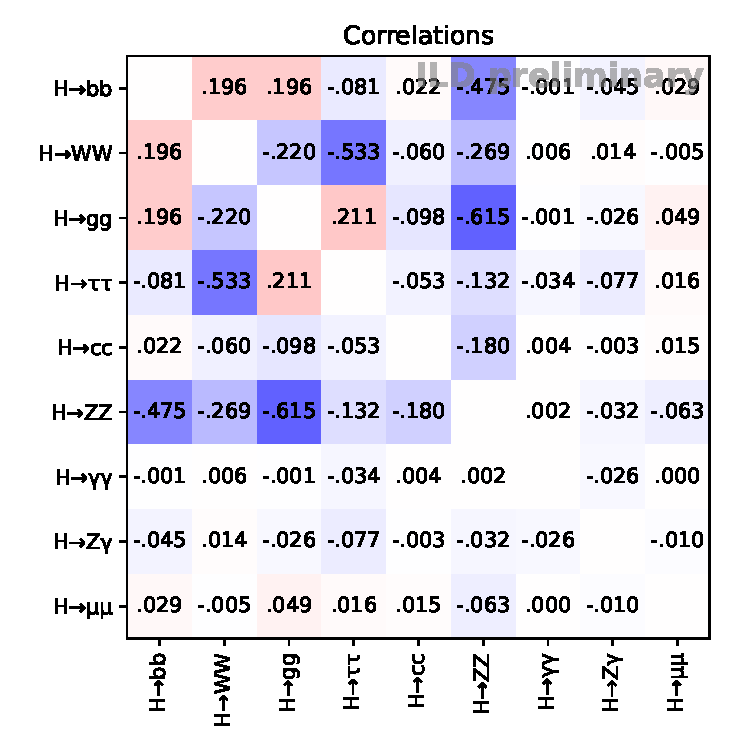
\includegraphics[width=\textwidth]{correlations}
        \caption{Correlations from \texttt{MINUIT} multinomial likelihood minimization.}
        \label{fig:correlations}
    \end{minipage}
    \end{figure}
    \begin{table}
        \resizebox{\textwidth}{!}{
            \InputBiasTable{bias_table.tex}
        }
        \caption{Fit on the
            expected event counts. In percent. ILD preliminary.}\label{tab:brs}
    \end{table}
\end{column}
\end{columns}
\end{block}
